%% Autor: Björn Ritterbecks 
%% Letzte Aenderung: 15.06.2016 
\thisfloatsetup{%
  capbesidewidth=\marginparwidth}
\begin{figure}[htbp]
\centering
%\sansmath
 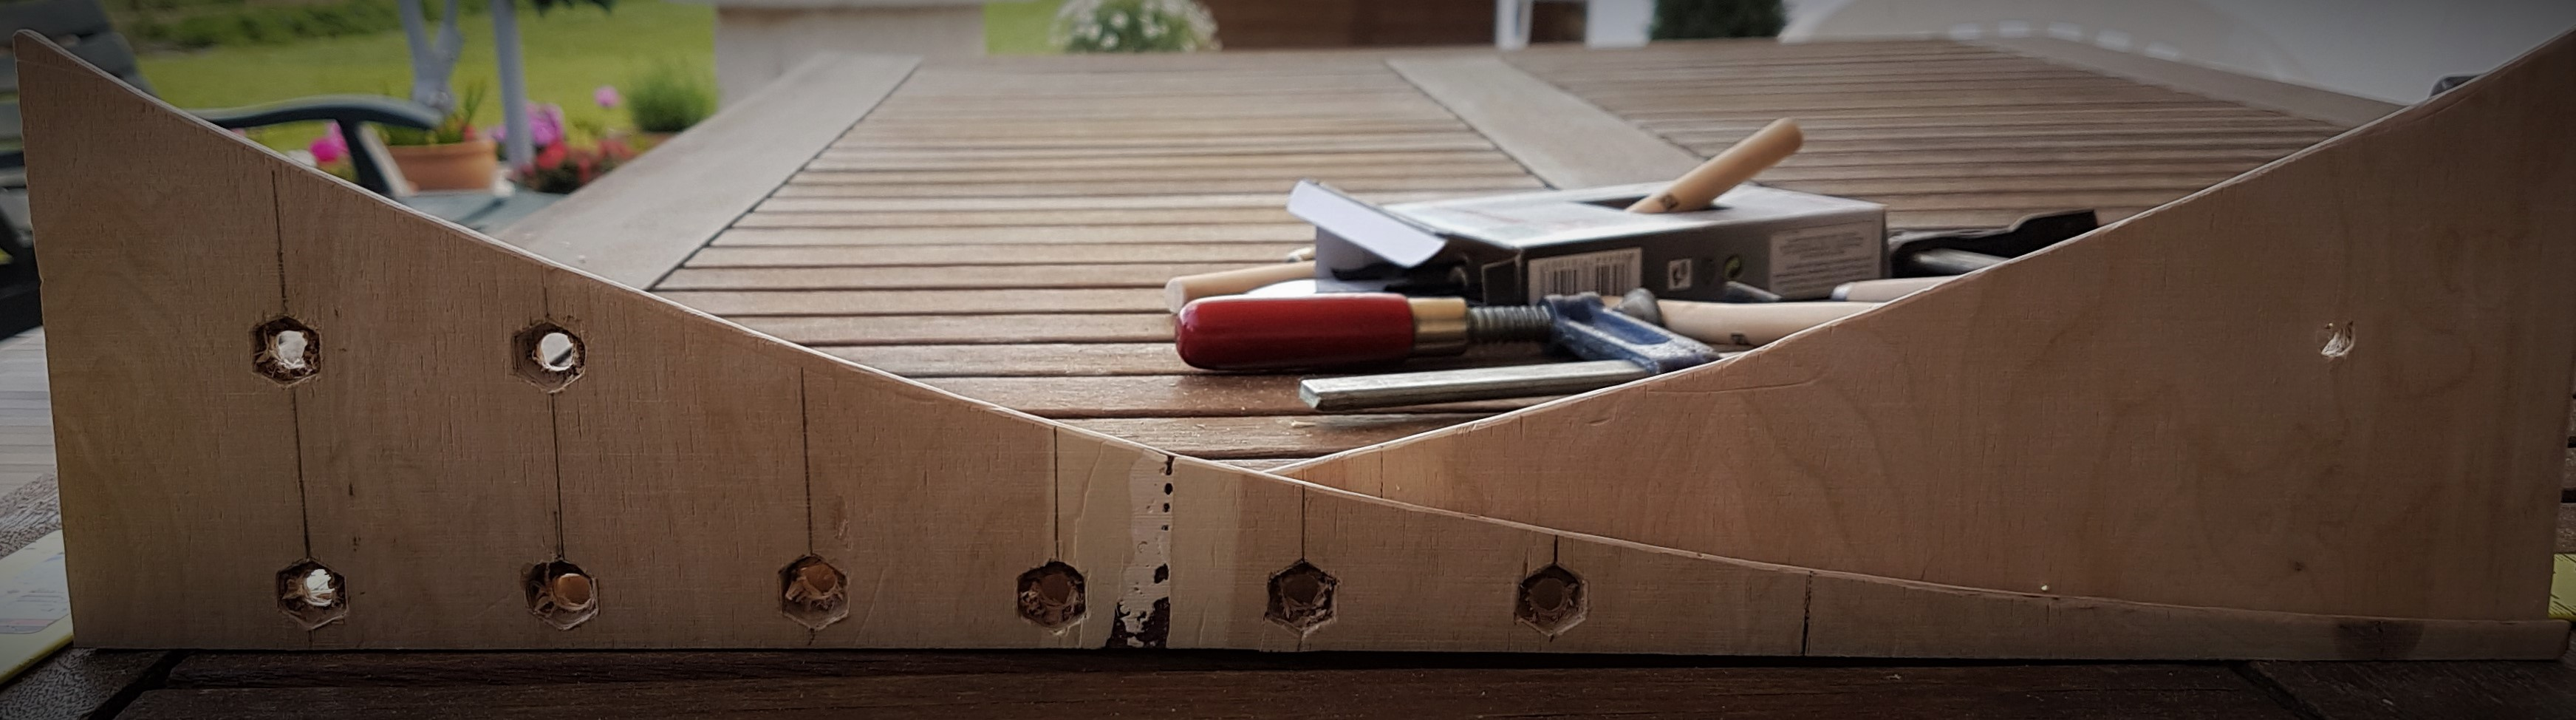
\includegraphics[width=0.99\textwidth]{images/rampenschliff1.jpg}
  \caption[Gesägte und gehobelte Rampensegmente]{Seitenansicht der gebauten Rampensegmente. Mittels eines nicht dehnbaren Fadens, Winkeln und einigen Schraubzwingen wird die Form angezeichnet und anschließend auf der Abfallseite ausgesägt. Die Annäherung an die endgültige Form erfolgt durch einen fein eingestellten Schweifhobel. Nach dem Durchbohren mit einem $\SI{6}{\milli\metre}$ Bohrer werden die Aussparungen für die Mutteraufnahme mit einem Stechbeitel gefertigt.}
  \label{fig:rampenschliff1}
  \vspace{-0pt}
\end{figure}